\documentclass[12pt]{article}
\usepackage[utf8]{inputenc}
\usepackage{mathtools}
\usepackage{amsmath}
\usepackage{derivative}
\usepackage{amsthm}
\usepackage{amssymb}
\usepackage{listings}
\usepackage{hyperref}
\usepackage{tikz}
\usepackage{float}
\usetikzlibrary{arrows,decorations.pathmorphing,backgrounds,positioning,fit,matrix}
\usepackage[symbols,nogroupskip,record]{glossaries-extra}
\usepackage[
backend=biber,
style=alphabetic,
sorting=ynt
]{biblatex}
\addbibresource{references.bib}

\glsxtrnewsymbol[
 description={position},
 location={(see chapter~\ref{ch1}).}
]{x}{\ensuremath{x}}
\glsxtrnewsymbol[description={velocity}]{v}{\ensuremath{v}}
\glsxtrnewsymbol[description={acceleration}]{a}{\ensuremath{a}}
\glsxtrnewsymbol[description={time}]{t}{\ensuremath{t}}
\glsxtrnewsymbol[description={force}]{F}{\ensuremath{F}}

\title{Investigating Car Following Model}
\author{Kaeshav Danesh and Kevin Phan}
\date{\today}

\begin{document}
    \maketitle

    \begin{abstract}
        Traffic flow dynamics is generally split into either macroscopic models or microscopic models. For this paper, we will focus on car following models which is a type of microscopic model. We first introduce the assumptions and the mathematical description car following model and the numerical scheme used to compute them. Then, we give the full velocity difference model. Finally, we examine different scenarios such as car crashes, phantom traffic, traffic light, and lane changes and analyze the behavior of cars. 
    \end{abstract}

    \tableofcontents

    \section{Introduction}
    

    \section{General Model}
    \subsection{Mathematical Formulation}\label{ch1}
        We follow the mathematical formulation of car following model in \cite{traffic}.
        \begin{figure}[H]
            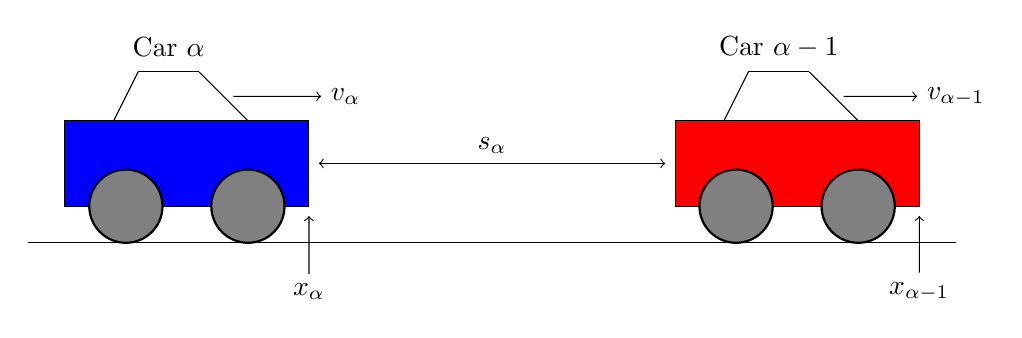
\begin{tikzpicture}[scale=1.55]
                \draw (-0.3,-0.3) -- (7.3,-0.3);
                \draw [fill = blue] (0,0) rectangle (2,0.7);
                \draw [fill=gray, thick] (0.5,0) circle [radius=0.3];
                \draw [fill=gray, thick] (1.5,0) circle [radius=0.3];
                \draw (1.5,0.7) -- (1.1,1.1);
                \draw (1.1,1.1) -- (0.6,1.1);
                \draw (0.6,1.1) -- (0.4,0.7);
                \node (car_a-1) at (0.85,1.3) {Car $\alpha$};
                \node (vel) at (2.3,0.9) {$v_{\alpha}$};
                \node (vel_start) at (1.3,0.9) {};
                \draw[->] (vel_start) -> (vel);
                \begin{scope}[shift={(5,0)}]
                    \draw [fill = red] (0,0) rectangle (2,0.7);
                    \draw [fill=gray, thick] (0.5,0) circle [radius=0.3];
                    \draw [fill=gray, thick] (1.5,0) circle [radius=0.3];
                    \draw (1.5,0.7) -- (1.1,1.1);
                    \draw (1.1,1.1) -- (0.6,1.1);
                    \draw (0.6,1.1) -- (0.4,0.7);
                    \node (car_a-1) at (0.85,1.3) {Car $\alpha - 1$};
                    \node (vel) at (2.3,0.9) {$v_{\alpha - 1}$};
                    \node (vel_start) at (1.3,0.9) {};
                    \draw[->] (vel_start) -> (vel);
                  \end{scope}
                \node (x) at (2,0.35) {};
                \node (y) at (5,0.35) {};
                \node (x_pos) at (2,0) {};
                \node (x_sym) at (2,-0.7) {$x_{\alpha }$};
                \node (x_pos1) at (7,0) {};
                \node (x_sym1) at (7,-0.7) {$x_{\alpha - 1}$};
                \draw[<->] (x) -- node[above] {$s_{\alpha}$} (y);
                \draw[<-] (x_pos) -- (x_sym);
                \draw[<-] (x_pos1) -- (x_sym1);
                \end{tikzpicture} 
            \centering
            \caption{Defining index, position, velocity, and gap of a car.}
        \end{figure}  


    \subsection{Numerical Scheme}
    \section{Car Following Model}
    \subsection{Full Velocity Difference Model}
    \section{Examining Different Scenarios}
    \subsection{Car Crash}
    \subsection{Phantom Traffic}
    \subsection{Traffic Light}
    \subsection{Lane Changes}
    \section{Conclusion}
    \section{Further Remarks}
    \printunsrtglossary[type=symbols,style=long,title={List of Symbols}]
    \newpage 
    \printbibliography
\end{document}